\documentclass[11pt,letterpaper]{article}
\PassOptionsToPackage{hyphens}{url}
\usepackage[margin=.83in,top=.8in,bottom=.8in,headheight=15pt]{geometry}
\usepackage[T1]{fontenc}
\usepackage{lmodern,amsmath,amssymb,mathtools,bm,booktabs,array,graphicx,tikz}
\usetikzlibrary{arrows.meta,positioning,calc,decorations.pathreplacing,patterns}
\definecolor{ink}{HTML}{17344D}\definecolor{accent}{HTML}{087E8B}\definecolor{pale}{HTML}{EDF5F5}\definecolor{gold}{HTML}{AD6B19}
\providecommand{\dd}{\,\mathrm{d}}\providecommand{\R}{\mathbb{R}}
\providecommand{\E}{\mathbb{E}}\providecommand{\Var}{\operatorname{Var}}
\providecommand{\Cov}{\operatorname{Cov}}\providecommand{\diag}{\operatorname{diag}}
\providecommand{\norm}[1]{\left\lVert#1\right\rVert}
\providecommand{\abs}[1]{\left|#1\right|}
\usepackage{microtype,hyperref,fancyhdr,enumitem,amsthm,sectsty,needspace}
\allsectionsfont{\raggedright}
\hypersetup{colorlinks=true,linkcolor=ink,urlcolor=accent,pdfauthor={Zan Ahmad},pdftitle={Least squares, principal components, and clustering / Lecture notes}}
\setlength{\parindent}{0pt}\setlength{\parskip}{6pt}\linespread{1.07}
\setlist{itemsep=3pt,topsep=4pt,leftmargin=*}
\emergencystretch=2em\clubpenalty=10000\widowpenalty=10000
\pagestyle{fancy}\fancyhf{}\fancyhead[L]{\small Scientific Computing in Python}\fancyhead[R]{\small Lecture 5}
\fancyfoot[L]{\footnotesize Zan Ahmad}\fancyfoot[R]{\footnotesize\thepage}\renewcommand{\headrulewidth}{.3pt}
\newtheorem{proposition}{Proposition}\newtheorem{theorem}{Theorem}\newtheorem{lemma}{Lemma}
\theoremstyle{definition}\newtheorem{definition}{Definition}\newtheorem{example}{Example}
\numberwithin{equation}{section}
\begin{document}
{\small\scshape Scientific Computing in Python\hfill Lecture 5}\par\medskip
{\raggedright\hyphenpenalty=10000\exhyphenpenalty=10000\LARGE\bfseries\color{ink} Least squares, principal components, and clustering\par}\medskip
{\small Lecture notes}\par\bigskip
A dataset can be used to estimate a response, represent variation in fewer coordinates, or partition observations by distance. These operations solve different optimization problems. We derive each objective and then examine how the choice of units and the train/test split enter the calculation.

\section{Linear least squares}
\hypertarget{note-linear-least-squares}{}\label{note:linear-least-squares}
{\small \href{slides.html\#frame=linear-least-squares\&step=1}{Slides for this section}}\par
For observations $(x_i,y_i)$, let $A$ have rows $(1,x_i)$ and let $\beta=(\beta_0,\beta_1)^{\mathsf T}$. Least squares minimizes the squared Euclidean distance between observed and fitted responses. Differentiation gives the normal equations. In computation a QR or SVD solve avoids explicitly forming an inverse.

\[
J(\beta)=\|A\beta-y\|_2^2.
\]

\[
\nabla J=2A^{\mathsf T}(A\beta-y)=0
\quad\Longrightarrow\quad A^{\mathsf T}A\beta=A^{\mathsf T}y.
\]

\subsection*{Residual orthogonality}
At a least-squares minimizer,
\[
A^{\mathsf T}r=0,\qquad r=A\widehat\beta-y.
\]

With an intercept column, $\sum_i r_i=0$ on the training set. There is no corresponding identity for held-out residuals.
\section{Units of a regression coefficient}
\hypertarget{note-units-of-a-regression-coefficient}{}\label{note:units-of-a-regression-coefficient}
{\small \href{slides.html\#frame=units-of-a-regression-coefficient\&step=1}{Slides for this section}}\par
The intercept has the response unit. A slope has response units divided by predictor units. Changing predictor units changes the numerical slope but should preserve predictions if coefficients are transformed consistently. The fitted relationship does not by itself establish a causal mechanism.

\[
\widehat y=\beta_0+\beta_1x.
\]
If $x'=ax$ with $a\ne0$, then

\[
\widehat y=\beta_0+\frac{\beta_1}{a}x'.
\]

\subsection*{Training and test error}
\[
\operatorname{RMSE}_{\rm test}=\sqrt{\frac1{n_{\rm test}}\sum_{i\in\rm test}(y_i-\widehat y_i)^2}.
\]

Fit the coefficients using training rows only. Test RMSE has the same physical unit as $y$.
\section{Principal component directions}
\hypertarget{note-principal-component-directions}{}\label{note:principal-component-directions}
{\small \href{slides.html\#frame=principal-component-directions\&step=1}{Slides for this section}}\par
Let $X_c$ be a data matrix whose columns have been centered using training means. A unit vector $v$ specifies a one-dimensional projection $z=X_cv$. Principal component analysis chooses the direction with maximal squared projected variation. A Lagrange multiplier converts the constrained optimization into an eigenvalue problem.

\[
\max_{v^{\mathsf T}v=1}\|X_cv\|_2^2.
\]

\[
X_c^{\mathsf T}X_cv=\lambda v.
\]
The leading eigenvector supplies the first principal direction.

\subsection*{Projection and reconstruction}
\[
z=(x-\mu)v_1,\qquad \widehat x=\mu+zv_1^{\mathsf T}.
\]

The reconstruction error is orthogonal to $v_1$. A large retained variance need not preserve information useful for predicting a separate response.
\begin{center}\begin{minipage}{.98\linewidth}\centering
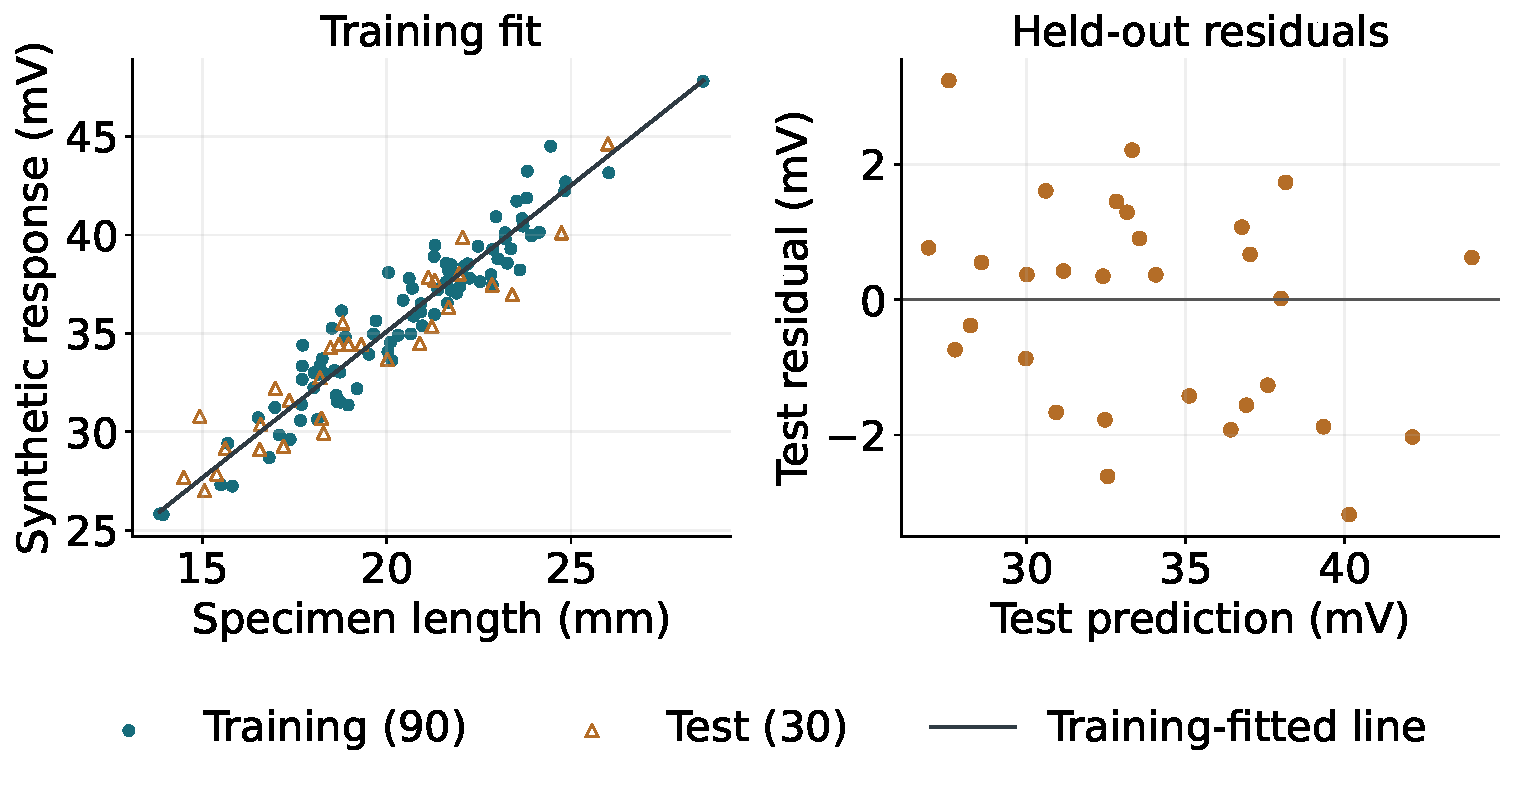
\includegraphics[width=.96\linewidth,height=.57\textheight,keepaspectratio]{regression-and-residuals.pdf}\par\smallskip
{\small Ninety training rows determine the line. Thirty held-out rows determine the displayed test residuals; response and residual units are millivolts.}
\end{minipage}\end{center}
\section{Scaling and distance}
\hypertarget{note-scaling-and-distance}{}\label{note:scaling-and-distance}
{\small \href{slides.html\#frame=scaling-and-distance\&step=1}{Slides for this section}}\par
Euclidean distance adds squared coordinate differences. Changing a mass column from grams to milligrams multiplies its squared contribution by a million. Training standardization replaces each coordinate by its deviation from the training mean divided by the training standard deviation. The same means and scales must then be used on test data.

\[
d^2(x,x')=\sum_j(x_j-x'_j)^2.
\]

\[
z_j=\frac{x_j-\mu_{j,\rm train}}{s_{j,\rm train}},\qquad s_{j,\rm train}>0.
\]

\subsection*{A zero-variance coordinate}
If $s_{j,\rm train}=0$, division is undefined.

A fixed rule must remove or separately handle that coordinate. Test data must not determine the training scale.
\Needspace{10\baselineskip}
\section{The k-means objective}
\hypertarget{note-the-k-means-objective}{}\label{note:the-k-means-objective}
{\small \href{slides.html\#frame=the-k-means-objective\&step=1}{Slides for this section}}\par
For a fixed number of centers, k-means minimizes within-group squared distances. Given centers, each observation is assigned to its nearest center. Given assignments, each center is the arithmetic mean of its assigned observations. Alternating these steps cannot increase the objective, but may converge to different local minima from different initializations.

\[
J(c,\mu)=\sum_i\|x_i-\mu_{c_i}\|_2^2.
\]

\[
c_i=\arg\min_k\|x_i-\mu_k\|_2^2,\qquad
\mu_k=\frac1{|C_k|}\sum_{i\in C_k}x_i.
\]

\subsection*{Group labels}
Permuting the center labels leaves the objective unchanged.

Group 0 and group 1 have no intrinsic biological meaning. Interpretation requires information beyond the distance calculation. The centroid formula assumes $|C_k|>0$. An empty cluster has no empirical mean and requires a specified reinitialization or reassignment rule.
\begin{center}\begin{minipage}{.98\linewidth}\centering
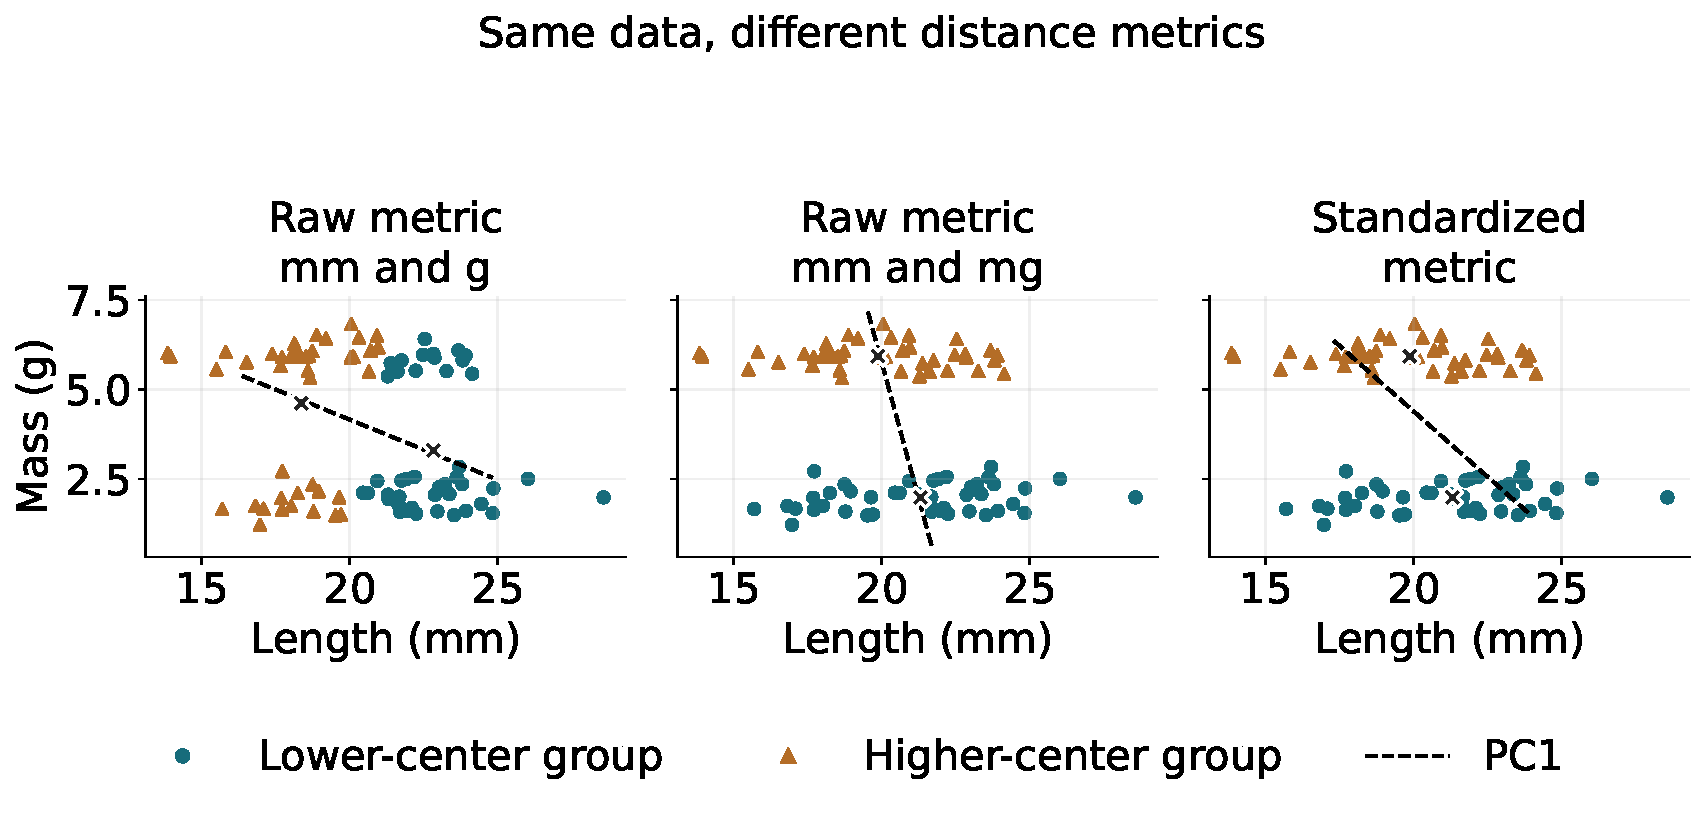
\includegraphics[width=.96\linewidth,height=.57\textheight,keepaspectratio]{scale-projection-groups.pdf}\par\smallskip
{\small All panels display length in millimeters and mass in grams. Computation uses raw mm/g, raw mm/mg, or training-standardized coordinates; dashed lines are PC1 and colors are fitted groups. Circle and triangle markers redundantly distinguish the groups ordered by center mass.}
\end{minipage}\end{center}
\Needspace{10\baselineskip}
\section{Fitted transformations and evaluation}
\hypertarget{note-fitted-transformations-and-evaluation}{}\label{note:fitted-transformations-and-evaluation}
{\small \href{slides.html\#frame=training-and-test-error\&step=1}{Slides for this section}}\par
A preprocessing step is part of the fitted model when it estimates means, scales, directions, or centers from data. It must be learned on the training subset. Fitting preprocessing on the full dataset allows test observations to influence the representation and changes the meaning of a held-out evaluation.

\[
\text{training data}\ \longmapsto\ (\mu,s,v_1,\widehat\beta,\widehat\mu_k).
\]

The fitted quantities are then held fixed when transforming and evaluating test observations.

\subsection*{A numerical implementation}
\begin{minipage}{\linewidth}
\begin{verbatim}
beta = np.linalg.lstsq(A_train, y_train, rcond=None)[0]
y_pred = A_test @ beta
rmse = np.sqrt(np.mean((y_test-y_pred)**2))
\end{verbatim}
\end{minipage}
No test response enters the coefficient solve.
\bigskip
\section*{Exercises}
\par\noindent\begin{minipage}{\linewidth}
\subsection*{H5-1. A line and a held-out residual}
Training lengths are [0, 1, 2] mm and responses [2, 4, 6] mV. A test specimen has length 3 mm and observed response 9 mV. New practice; 10 feedback points.

\textbf{a} Find a line that exactly fits training data and state coefficient units.

\end{minipage}\par\medskip
\textbf{b} Compute the test prediction, observed-minus-predicted residual and single-test-point RMSE.

\textbf{c} Compare the training-mean baseline and explain why zero training error does not settle test performance.

\par\noindent\begin{minipage}{\linewidth}
\subsection*{H5-2. Project and reconstruct}
Centered feature rows are [-2, 0], [0, 0] and [2, 0]. Treat both coordinates as dimensionless. New practice; 10 feedback points.

\textbf{a} Give a first principal direction and the three one-component scores. Explain why this direction captures all variation and describe its sign ambiguity.

\end{minipage}\par\medskip
\textbf{b} Reconstruct the rows from those scores and state the reconstruction error.

\textbf{c} Would perfect feature reconstruction prove that the scores predict an unrelated response?

\par\noindent\begin{minipage}{\linewidth}
\subsection*{H5-3. Units and preprocessing}
A centered two-feature table has numerical covariance diag(4, 1), with zero cross-covariance. New practice; 10 feedback points.

\textbf{a} Identify the leading raw PCA coordinate, then multiply the second feature by three and identify the new leading coordinate.

\end{minipage}\par\medskip
\textbf{b} A training feature has mean 10 and standard deviation 2. Standardize a test value of 14. Explain why its test-set mean should not replace 10.

\textbf{c} Does standardization prove the best scientific weighting or a unique PCA direction?

\par\noindent\begin{minipage}{\linewidth}
\subsection*{H5-4. Trace a two-center update}
Four dimensionless one-feature rows are 0, 1, 7 and 8. Initial centers are 0 and 8. New practice; 10 feedback points.

\textbf{a} Assign each row to its nearest center and compute updated centers.

\end{minipage}\par\medskip
\textbf{b} Compute the within-group squared-distance sum before and after the update. Explain why replacing each center by its fixed-assignment group mean lowers the objective here.

\textbf{c} Explain why swapping group labels does not change this result and why the two groups are not automatically known classes.

\section*{References}
\noindent\begin{minipage}{\linewidth}
Original Python Lecture 5. PDF pages 5--18.

\url{https://zanahmad.com/files/scientific-python/Lecture_5__Intro_to_Python.pdf}
\end{minipage}\par\medskip
\noindent\begin{minipage}{\linewidth}
NumPy least-squares reference. Parameters, returned rank and residuals.

\url{https://numpy.org/doc/stable/reference/generated/numpy.linalg.lstsq.html}
\end{minipage}\par\medskip
\noindent\begin{minipage}{\linewidth}
NumPy singular-value decomposition reference. Reduced two-dimensional factorization and returned factors.

\url{https://numpy.org/doc/stable/reference/generated/numpy.linalg.svd.html}
\end{minipage}\par\medskip
\noindent\begin{minipage}{\linewidth}
scikit-learn PCA guide. Section 2.5.1.1: centering, scaling and principal directions.

\url{https://scikit-learn.org/stable/modules/decomposition.html#pca}
\end{minipage}\par\medskip
\noindent\begin{minipage}{\linewidth}
scikit-learn clustering guide. Section 2.3.2: centroid objective, alternating steps and local minima.

\url{https://scikit-learn.org/stable/modules/clustering.html#k-means}
\end{minipage}\par\medskip
\noindent\begin{minipage}{\linewidth}
scikit-learn common pitfalls. Sections 12.1--12.2.1: consistent preprocessing and training-only fitting.

\url{https://scikit-learn.org/stable/common_pitfalls.html#data-leakage}
\end{minipage}\par\medskip
Python source materials: Phillip Kerger (2023). Course adaptation and additional exposition: Zan Ahmad.

\end{document}
